% Inicialização do relatório e importação dos módulos necessários
\documentclass[a4paper,12pt]{article}
\usepackage[T1]{fontenc}
\usepackage{graphicx}
\usepackage{titling}
\usepackage{tcolorbox}
\usepackage{listings}
\usepackage{color}
\usepackage{caption}

% Criação do título do relatório
\pretitle{
        \begin{center}
        \LARGE
        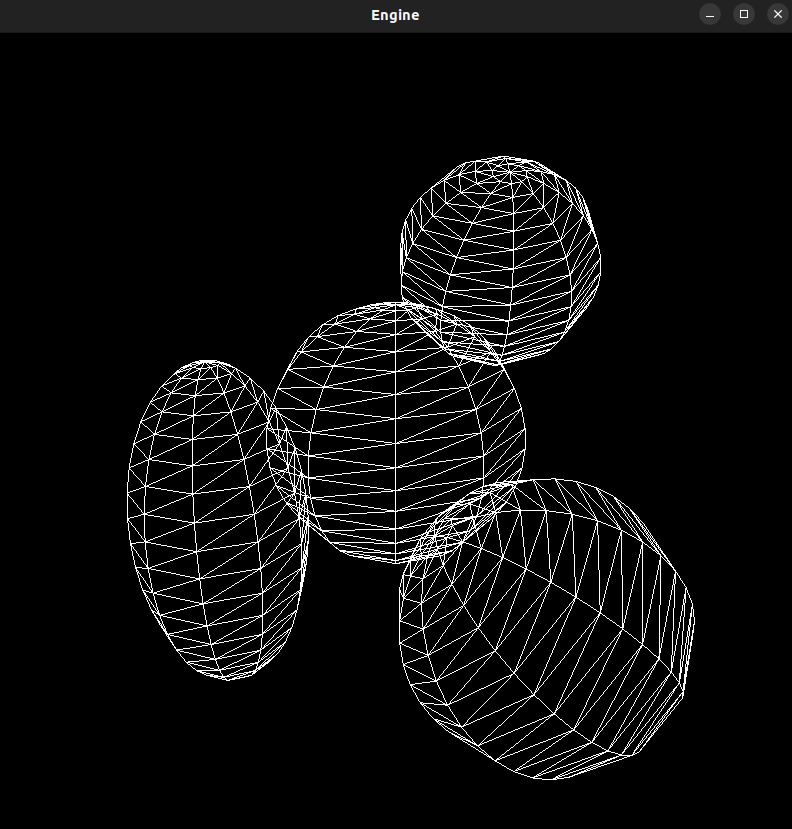
\includegraphics[width=10cm]{imgs/capa.png}\\[\bigskipamount]
        \title{\textbf{Computação Gráfica - Relatório 2ª Fase}}
        \author{Gabriel Pereira, a100891\\
                Guilherme Oliveira, a100592\\
                Gustavo Castro, a100482}
}

% Definição do estilo do relatório
\lstdefinestyle{BASH}
{
        backgroundcolor=\color{black},
        basicstyle=\scriptsize\color{white}\ttfamily     
}

% Definição da posição do título
\posttitle{
        \end{center}
}

% Inicialização do documento
\begin{document}

% Impressão do título do documento
\begin{titlepage}
        \pagenumbering{gobble}
        \maketitle
\end{titlepage}

% Numeração das páginas
\pagenumbering{arabic}

% Secção de Introdução do Relatório
\section{Introdução}
\noindent
É pretendida a expansão do motor gráfico implementado na
fase anterior, tal que este consiga, para além de
representar primitivas, fazer transformações nas mesmas.
\newline
\break
\noindent
Para além disso, o motor deverá, ainda, ser capaz de
suportar a existência de sub-grupos, que deverão herdar as
transformações do grupo a que pertencem.
\newline
\break
\noindent
Estas transformações e grupos terão, portanto, de ser
definidas, à semelhança da primeira fase, na configuração
dada em formato \textbf{XML} e o motor deverá ser capaz
de ler e armazená-las em memória para,
posteriormente, as representar.


% Secção dos Requisitos do Solução
\section{Requisitos}
Definidos os objetivos para esta fase da implementação,
especificaram-se requisitos, garantias e funcionalidades
que a arquitetura deverá respeitar.
\newline
\break
\noindent
Em constrate com a fase inicial desta solução, para
garantir a implementação pretendida apenas será
necessário atualizar o motor gráfico, que agora deverá
conseguir identificar transformações e sub-grupos.

\subsection{Transformações}

O motor gŕafico terá, portanto, a necessidade de
conseguir identificar e armazenar todos os tipos
de transformações existentes.
\newline
\break
\noindent
Existem três tipos de transformações:
\textbf{translações, rotações e escalas} e cada uma delas
apresenta um conjunto de propriedades que permitem
definir como a primitiva será afeta por elas.
\newline

\begin{tcolorbox}[
    colback=blue!10!white,
    colframe=black!50!black,
]
\begin{verbatim}
Translação:
    x, y, z -> translação sobre os eixos x, y, z

Rotação:
    angle -> ângulo de rotação
    x, y, z -> eixo de rotação definido

Scale:
    x, y, z -> escala sobre os eixos x, y, z
\end{verbatim}
\end{tcolorbox}

\vspace{12pt}
\noindent
Estas transformações devem, então, ser definidas numa
configuração \textbf{XML} envolvidas sob uma etiqueta
\textbf{Transform}, que inicia um grupo de
transformações.
\newline
\break
\noindent
Dentro de um grupo não é permitido, também,
existir repetições de um mesmo tipo de transformação,
ou seja, se um grupo já possuí uma translação, uma outra
translação apenas pode ser definida noutro grupo ou
sub-grupo.
\newline
\break
\noindent
A configuração assume, portanto, o seguinte
formato exemplar:
\newline

\begin{tcolorbox}[
    colback=blue!10!white,
    colframe=black!50!black,
    after upper={\hfill\textbf{xml}}
]
\begin{verbatim}
<world>
    <window width="512" height="512" />
    <camera>
        <position x="10" y="10" z="10" />
        <lookAt x="0" y="0" z="0" />
        <up x="0" y="1" z="0" />
        <projection fov="60" near="1" far="1000" />
    </camera>
    <group>
        <transform>
            <translate x="4" y="0" z="0" />
            <rotate angle="30" x="0" y="1" z="0" />
            <scale x="2" y="0.3" z="1" />
        </transform>
        <models>
            <model file="cone.3d" />
            <model file="plane.3d" />
        </models>
    </group>
</world>
\end{verbatim}
\end{tcolorbox}

% Secção de Conceptualização da Solução
\section{Conceptualização}
Estabelecidos os requisitos pretendidos para a
implementação, foram atualizados os modelos conceptuais
de forma a sustentar as novas funcionalidades pretendidas.
\newline

\subsection{Gerador de Primitivas}

\begin{center}
    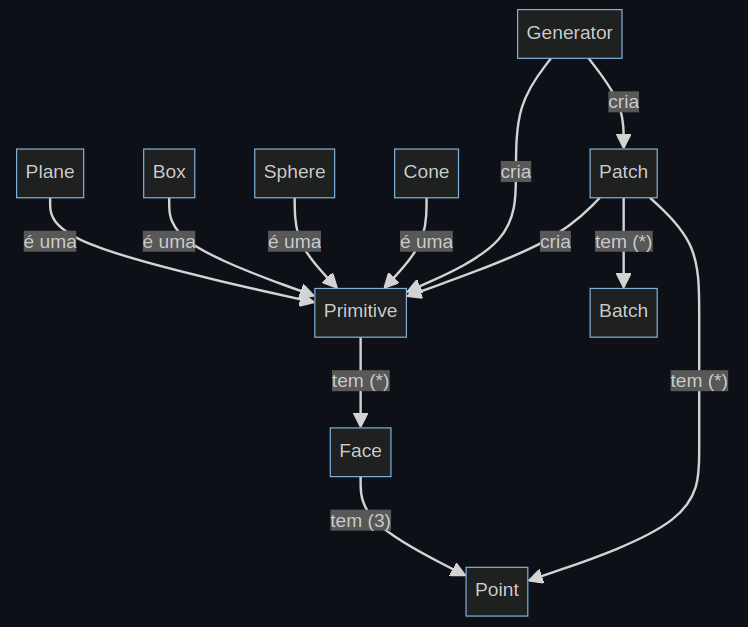
\includegraphics[width=0.8\textwidth]{imgs/concept1.png}
    \captionof{figure}{Modelo de Domínio do Gerador de Primitivas}
    \label{fig:domger}
\end{center}

\noindent
No gerador de primitivas as diferenças são mais notórias na parte
da implementação do que na arquitetura, visto que o maior papel
desta componente é realizar cálculos.\\
\\
Porém, ainda assim existem alguns componentes arquiteturais
que foram utilizados para auxiliar ao cálculo, armazenamento
e escrita das novas propriedades.\\
\\
O ponto do gerador passará, portanto, para além das suas coordenadas,
a armazenar também as coordenadas da sua normal, assim como, das
suas texturas, através da estrutura \textbf{TextureCoordinates}
(que será também utilizada para o motor gráfico).

\subsection{Motor gráfico}

\begin{center}
    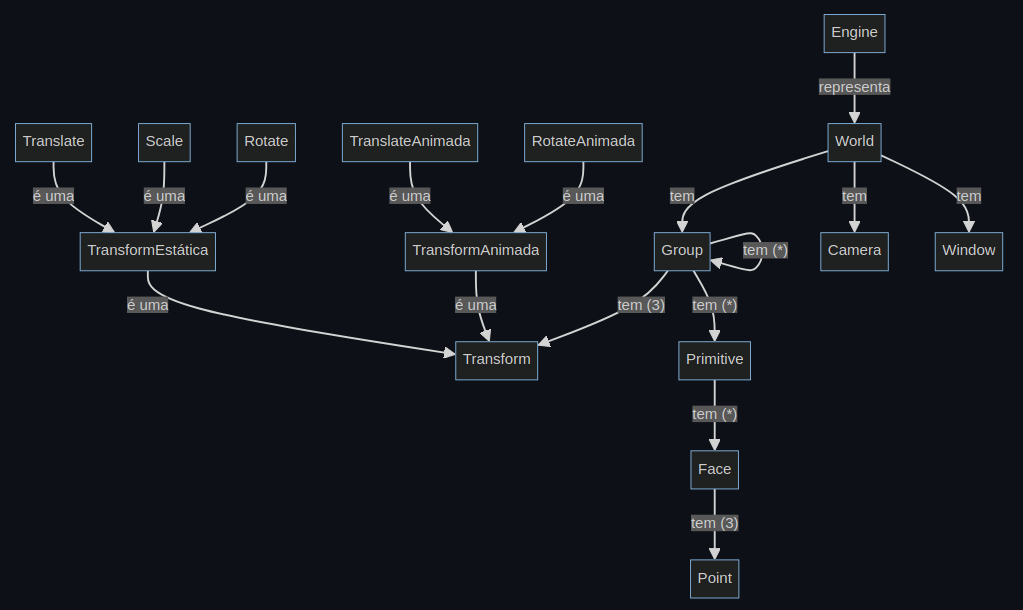
\includegraphics[width=1.0\textwidth]{imgs/concept2.png}
    \captionof{figure}{Modelo de Domínio do Motor Gráfico}
    \label{fig:domeng}
\end{center}

\noindent
Partindo da hierarquia até agora utilizada, o motor gráfico
teve algumas transformações notórias.\\
\\
Foram, portanto, esboçadas estruturas que suportem a definição
dos vários tipos de luz que deverão ser armazenadas num grupo
da configuração (como especificado nos requisitos).\\
\\
Estas estruturas conterão as propriedades necessárias para a
definição das luzes no cenário e deverão ser desenhadas após
as transformações do grupo serem aplicadas.\\
\\
Para além disso, deverão ser ativadas no início dos desenhos
do respetivo grupo e desativadas no final
do desenho do grupo (após o desenho dos sub-grupos), de forma
a cumprir o requisito e não
afetar outros grupos na mesma hierarquia.\\
\\
Ainda foram especificadas estruturas que pretendem armazenar
as componentes de cor e textura, pertencentes a uma primitiva.
A estrutura de cor é capaz de armazenar qualquer tipo de cor,
identificando o seu tipo nas suas propriedades e a estrutura
de textura guarda os índices necessários para a aplicação
de uma textura a um objeto.\\
\\
De forma a armazenar as normais, reutilizou-se a estrutura de
ponto, que, sendo constituída por três coordenadas e já ter
capacidade de leitura de ficheiros, rapidamente se encaixa
para este propósito. Para armazenar as coordenadas de textura,
reutilizou-se a estrutura já definida para o gerador.

% Secção de Implementação da Solução
\section{Implementação}
Definida a nova arquitetura e tendo as necessidades de
implementação em mente, foram, agora, tomadas algumas
decisões da implementação da arquitetura modificada.
\newline
\break
\noindent
Como especificado anteriormente, a arquitetura da 
transformação irá fazer uso de uma super-classe, que
deverá especificar que todas as suas sub-classes possuem
um método que permite à transformação definida ser
aplicada.
\newline
\break
\noindent
Estas transformações deverão, então, ser guardadas numa
lista de transformações do grupo de forma a manter a sua
ordem de aplicação (uma vez que o resultado é diferente
dependendo da ordem das transformações), onde não deverá
haver duas transformações do mesmo tipo.
\newline
\break
\noindent
Já a definição dos sub-grupos seguirá uma estratégia
semelhante, guardando os vários sub-grupos numa lista
de grupos. Cada grupo será, então, desenhado pela ordem
de aparição na configuração, fazendo uso da definição
recursiva para a função de desenho.
\newline
\break
\noindent
Por último, de forma a manter a herança de
transformações e evitar a sua aplicação indesejada,
o início do desenho de cada grupo será
o armazenamento da matriz atual, seguido da aplicação
das transformações, desenho dos modelos e dos grupos e,
posteriormente, de um restauro da matriz armazenada
inicialmente.

% Secção de Resultados da Solução
\section{Resultados}
Concluída a solução, foram construídas algumas cenas
tridimensionais, como de costume, que pretendem testar e exemplificar as funcionalidades
implementadas na solução obtida.
\newline
\break
\noindent
Estas cenas pretendem demonstrar o uso de \textbf{patches}
e transformações animadas de forma a melhorar modelos já construídos anteriormente.
\newline
\break
\noindent
Estas cenas podem, então, ser observados nas figuras
\ref{fig:snowman}, \ref{fig:solarlign} e \ref{fig:solar}.

\subsection{Boneco de Neve}

\begin{center}
    
\includegraphics[width=0.8\textwidth]{imgs/boneconeve.png}
    \captionof{figure}{Boneco de Neve construído com transformações}
    \label{fig:snowman}
\end{center}

\subsection{Sistema Solar Alinhado}

\begin{center}
    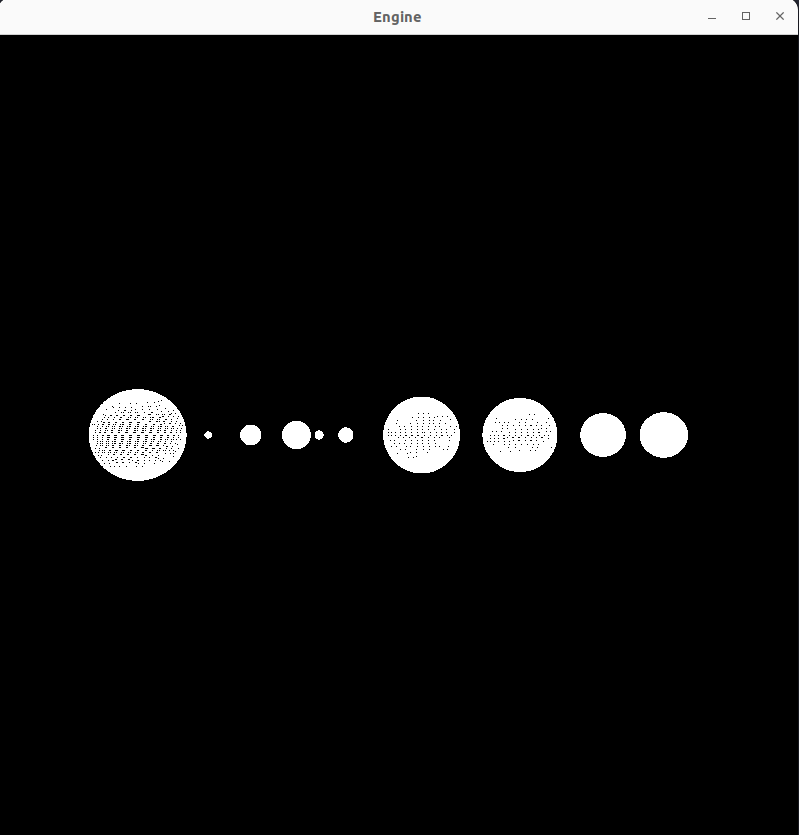
\includegraphics[width=0.8\textwidth]{imgs/sissolarhor.png}
    \captionof{figure}{Sistema Solar construído com transformações}
    \label{fig:solarlign}
\end{center}

\subsection{Sistema Solar}

\begin{center}
    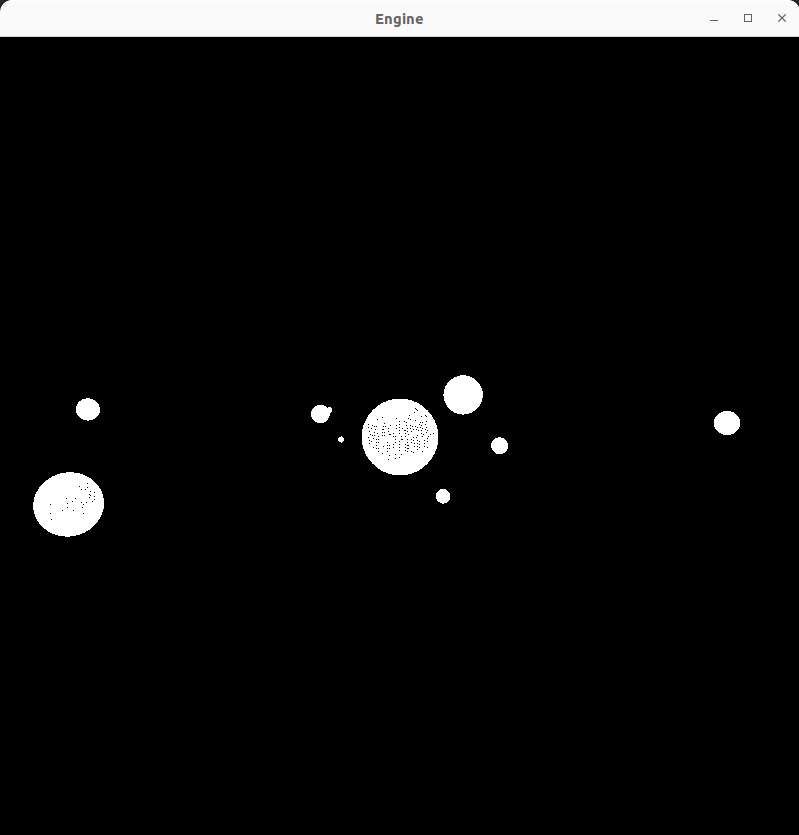
\includegraphics[width=0.8\textwidth]{imgs/sissolar.png}
    \captionof{figure}{Sistema Solar disperso construído com transformações}
    \label{fig:solar}
\end{center}



% Secção de Conclusão e Trabalho Futuro
\section{Conclusão e Trabalho Futuro}
Concluída, com sucesso, a última fase, a solução considera-se
terminada, apenas apresentando necessidades para poucas
melhorias (mais relativas a performance e alocação de
memória).

% Finalização do documento
\end{document}